% Created by tikzDevice version 0.12.3.1 on 2021-12-15 14:08:41
% !TEX encoding = UTF-8 Unicode
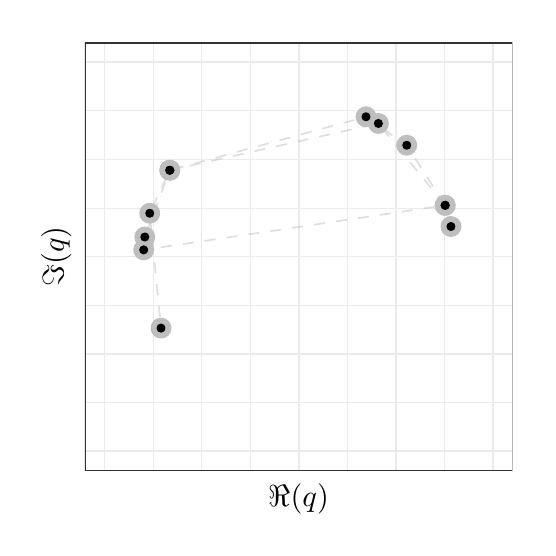
\begin{tikzpicture}[x=1pt,y=1pt]
\definecolor{fillColor}{RGB}{255,255,255}
\path[use as bounding box,fill=fillColor,fill opacity=0.00] (0,0) rectangle (180.67,180.67);
\begin{scope}
\path[clip] (  0.00,  0.00) rectangle (180.67,180.67);
\definecolor{drawColor}{RGB}{255,255,255}
\definecolor{fillColor}{RGB}{255,255,255}

\path[draw=drawColor,line width= 0.6pt,line join=round,line cap=round,fill=fillColor] (  0.00,  0.00) rectangle (180.67,180.68);
\end{scope}
\begin{scope}
\path[clip] ( 20.71, 20.71) rectangle (175.17,175.17);
\definecolor{fillColor}{RGB}{255,255,255}

\path[fill=fillColor] ( 20.71, 20.71) rectangle (175.17,175.17);
\definecolor{drawColor}{gray}{0.92}

\path[draw=drawColor,line width= 0.3pt,line join=round] ( 20.71, 45.29) --
	(175.17, 45.29);

\path[draw=drawColor,line width= 0.3pt,line join=round] ( 20.71, 80.39) --
	(175.17, 80.39);

\path[draw=drawColor,line width= 0.3pt,line join=round] ( 20.71,115.50) --
	(175.17,115.50);

\path[draw=drawColor,line width= 0.3pt,line join=round] ( 20.71,150.60) --
	(175.17,150.60);

\path[draw=drawColor,line width= 0.3pt,line join=round] ( 45.29, 20.71) --
	( 45.29,175.17);

\path[draw=drawColor,line width= 0.3pt,line join=round] ( 80.39, 20.71) --
	( 80.39,175.17);

\path[draw=drawColor,line width= 0.3pt,line join=round] (115.50, 20.71) --
	(115.50,175.17);

\path[draw=drawColor,line width= 0.3pt,line join=round] (150.60, 20.71) --
	(150.60,175.17);

\path[draw=drawColor,line width= 0.6pt,line join=round] ( 20.71, 27.74) --
	(175.17, 27.74);

\path[draw=drawColor,line width= 0.6pt,line join=round] ( 20.71, 62.84) --
	(175.17, 62.84);

\path[draw=drawColor,line width= 0.6pt,line join=round] ( 20.71, 97.94) --
	(175.17, 97.94);

\path[draw=drawColor,line width= 0.6pt,line join=round] ( 20.71,133.05) --
	(175.17,133.05);

\path[draw=drawColor,line width= 0.6pt,line join=round] ( 20.71,168.15) --
	(175.17,168.15);

\path[draw=drawColor,line width= 0.6pt,line join=round] ( 27.74, 20.71) --
	( 27.74,175.17);

\path[draw=drawColor,line width= 0.6pt,line join=round] ( 62.84, 20.71) --
	( 62.84,175.17);

\path[draw=drawColor,line width= 0.6pt,line join=round] ( 97.94, 20.71) --
	( 97.94,175.17);

\path[draw=drawColor,line width= 0.6pt,line join=round] (133.05, 20.71) --
	(133.05,175.17);

\path[draw=drawColor,line width= 0.6pt,line join=round] (168.15, 20.71) --
	(168.15,175.17);
\definecolor{drawColor}{RGB}{190,190,190}
\definecolor{fillColor}{RGB}{190,190,190}

\path[draw=drawColor,line width= 0.4pt,line join=round,line cap=round,fill=fillColor] (152.95,108.82) circle (  3.57);

\path[draw=drawColor,line width= 0.4pt,line join=round,line cap=round,fill=fillColor] (150.86,116.48) circle (  3.57);

\path[draw=drawColor,line width= 0.4pt,line join=round,line cap=round,fill=fillColor] (126.73,146.06) circle (  3.57);

\path[draw=drawColor,line width= 0.4pt,line join=round,line cap=round,fill=fillColor] ( 51.36,129.15) circle (  3.57);

\path[draw=drawColor,line width= 0.4pt,line join=round,line cap=round,fill=fillColor] ( 42.32,105.03) circle (  3.57);

\path[draw=drawColor,line width= 0.4pt,line join=round,line cap=round,fill=fillColor] ( 41.93,100.38) circle (  3.57);

\path[draw=drawColor,line width= 0.4pt,line join=round,line cap=round,fill=fillColor] (150.86,116.48) circle (  3.57);

\path[draw=drawColor,line width= 0.4pt,line join=round,line cap=round,fill=fillColor] (136.98,138.19) circle (  3.57);

\path[draw=drawColor,line width= 0.4pt,line join=round,line cap=round,fill=fillColor] (122.25,148.47) circle (  3.57);

\path[draw=drawColor,line width= 0.4pt,line join=round,line cap=round,fill=fillColor] ( 51.36,129.15) circle (  3.57);

\path[draw=drawColor,line width= 0.4pt,line join=round,line cap=round,fill=fillColor] ( 44.11,113.61) circle (  3.57);

\path[draw=drawColor,line width= 0.4pt,line join=round,line cap=round,fill=fillColor] ( 48.18, 72.11) circle (  3.57);
\definecolor{drawColor}{RGB}{190,190,190}

\path[draw=drawColor,draw opacity=0.50,line width= 0.6pt,dash pattern=on 4pt off 4pt ,line join=round] (152.95,108.82) --
	(150.86,116.48) --
	(126.73,146.06) --
	( 51.36,129.15) --
	( 42.32,105.03) --
	( 41.93,100.38) --
	(150.86,116.48) --
	(136.98,138.19) --
	(122.25,148.47) --
	( 51.36,129.15) --
	( 44.11,113.61) --
	( 48.18, 72.11);
\definecolor{drawColor}{RGB}{0,0,0}
\definecolor{fillColor}{RGB}{0,0,0}

\path[draw=drawColor,line width= 0.4pt,line join=round,line cap=round,fill=fillColor] (152.95,108.82) circle (  1.43);

\path[draw=drawColor,line width= 0.4pt,line join=round,line cap=round,fill=fillColor] (150.86,116.48) circle (  1.43);

\path[draw=drawColor,line width= 0.4pt,line join=round,line cap=round,fill=fillColor] (126.73,146.06) circle (  1.43);

\path[draw=drawColor,line width= 0.4pt,line join=round,line cap=round,fill=fillColor] ( 51.36,129.15) circle (  1.43);

\path[draw=drawColor,line width= 0.4pt,line join=round,line cap=round,fill=fillColor] ( 42.32,105.03) circle (  1.43);

\path[draw=drawColor,line width= 0.4pt,line join=round,line cap=round,fill=fillColor] ( 41.93,100.38) circle (  1.43);

\path[draw=drawColor,line width= 0.4pt,line join=round,line cap=round,fill=fillColor] (150.86,116.48) circle (  1.43);

\path[draw=drawColor,line width= 0.4pt,line join=round,line cap=round,fill=fillColor] (136.98,138.19) circle (  1.43);

\path[draw=drawColor,line width= 0.4pt,line join=round,line cap=round,fill=fillColor] (122.25,148.47) circle (  1.43);

\path[draw=drawColor,line width= 0.4pt,line join=round,line cap=round,fill=fillColor] ( 51.36,129.15) circle (  1.43);

\path[draw=drawColor,line width= 0.4pt,line join=round,line cap=round,fill=fillColor] ( 44.11,113.61) circle (  1.43);

\path[draw=drawColor,line width= 0.4pt,line join=round,line cap=round,fill=fillColor] ( 48.18, 72.11) circle (  1.43);
\definecolor{drawColor}{gray}{0.20}

\path[draw=drawColor,line width= 0.6pt,line join=round,line cap=round] ( 20.71, 20.71) rectangle (175.17,175.17);
\end{scope}
\begin{scope}
\path[clip] (  0.00,  0.00) rectangle (180.67,180.67);
\definecolor{drawColor}{RGB}{0,0,0}

\node[text=drawColor,anchor=base,inner sep=0pt, outer sep=0pt, scale=  1.10] at ( 97.94,  7.64) {$\Re(q)$};
\end{scope}
\begin{scope}
\path[clip] (  0.00,  0.00) rectangle (180.67,180.67);
\definecolor{drawColor}{RGB}{0,0,0}

\node[text=drawColor,rotate= 90.00,anchor=base,inner sep=0pt, outer sep=0pt, scale=  1.10] at ( 13.08, 97.94) {$\Im(q)$};
\end{scope}
\end{tikzpicture}
